%% This demo file is intended to serve as a ``starter file'' for 
%% IEEE Journal of Electromagnetics, RF and Microwaves in Medicine and
       

\documentclass[journal,twocolumn,letterpaper]{IEEEJERM}
%
% If IEEEtran.cls has not been installed into the LaTeX system files,
% manually specify the path to it like:
% \documentclass[journal]{../sty/IEEEtran}


% *** GRAPHICS RELATED PACKAGES ***
%


\usepackage{times,amsmath,epsfig}
\usepackage{fancyhdr}
\usepackage{amsmath}
\usepackage{amsfonts}
\usepackage{amssymb}
\usepackage[latin1]{inputenc}
\usepackage{array}
\usepackage{graphicx}
\usepackage{url}
%\usepackage{subfigure}
\usepackage{bm}
\usepackage{breqn}
\usepackage{xcolor}
\usepackage{soul}
\usepackage{amssymb}
\usepackage{mathrsfs}
\usepackage{amsmath,amsthm,amsfonts,amssymb,amscd}
\usepackage{listings}
\usepackage[framed,numbered]{mcode}
% correct bad hyphenation here
\hyphenation{op-tical net-works semi-conduc-tor}
\usepackage{float}
\usepackage{booktabs}
%\usepackage{appendix}

\ifCLASSOPTIONcompsoc
\usepackage[caption=false, font=normalsize, labelfont=sf, textfont=sf]{subfig}
\else
\usepackage[caption=false, font=footnotesize]{subfig}

\begin{document}

%
% paper title
% Titles are generally capitalized except for words such as a, an, and, as,
% at, but, by, for, in, nor, of, on, or, the, to and up, which are usually
% not capitalized unless they are the first or last word of the title.
% Linebreaks \\ can be used within to get better formatting as desired.
% Do not put math or special symbols in the title.
\title{Matlab Simulation of Magnetic Focusing Model
}

%
% author names and IEEE memberships
% note positions of commas and nonbreaking spaces ( ~ ) LaTeX will not break
% a structure at a ~ so this keeps an author's name from being broken across
% two lines.
\author{Junlong~Huang~11810405,
	
	~\IEEEmembership{Southern University of Science and Technology}
}% <-this % stops a space

% The paper headers
\markboth{IEEE Journal of Electromagnetics, RF and Microwaves in Medicine and Biology}
{Z. Peng \MakeLowercase{\textit{et al.}}: Demo of IEEE Journal of Electromagnetics, RF and Microwaves in Medicine and Biology (JERM)}


\twocolumn[
\begin{@twocolumnfalse}
  
% make the title area
\maketitle

% As a general rule, do not put math, special symbols or citations
% in the abstract or keywords.
\begin{abstract}
	Similar to a lens that focuses a light beam, magnetic focusing is a charged particle beam with a small divergence angle. When they have the same velocity component in the direction of the magnetic field, the divergent particle beam converges to a point after a period.  In this process, the analytical solution of the velocity and displacement vector at each moment can be obtained by solving the differential equation. However, this process is sometimes too tedious. In order to focus on understanding the physical nature of  magnetic focusing dynamic process, the Matlab is used to calculate and draw the movement trajectory of charge.
\end{abstract}

% Note that keywords are not normally used for peerreview papers.
\begin{IEEEkeywords}
 Lorentz force, Magnetic focusing, Matlab simulation.
\end{IEEEkeywords}

\end{@twocolumnfalse}]

\IEEEpeerreviewmaketitle


\section{Introduction}

\IEEEPARstart{T}{he} electric charge will be affected by the Lorentz force in the electromagnetic field. The charge will generate acceleration under the action of Lorentz force, which will produce changes in speed and displacement. In this process, the analytical solution of the velocity and displacement vector at each moment can be obtained by solving the differential equation. However, this process is sometimes too tedious and the result is not intuitive. For example, in magnetic focusing, the trajectory of particles often describes this phenomenon better than the equation of motion of particles.

Magnetic focusing is a charged particle beam with a small divergence angle. When they have the same velocity component in the direction of the magnetic field, the divergent particle beam converges to a point after a period. Magnetic focusing is widely used in fields such as electron microscopy.\cite{num3}

 In order to focus on understanding the physical nature of  magnetic focusing dynamic process, the movement trajectory of charge is calculated and drawn by Matlab. At the same time, the relevant parameters and properties of magnetic focusing have been verified.
 
\section{Method and Analysis}
\subsection{Mathematical calculation
}
Charge in magnetic field will be subject to the action of Lorentz force, which is expressed as:
\begin{align}
\vec{F}=q\vec{E}+q\vec{v}\times \vec{B}
\end{align}
where $ \vec{F} $ is vector of Lorentz force, $ \vec{E}$ is the vector of electron field, $ \vec{B} $ is the vector of magnetic flux density, $ \vec{v} $ is the vector of charge's velocity, $ q $ is the quantity of charge.

The electromagnetic field is written as a component in the plane rectangular coordinate system, which is:
\begin{align}
\vec{E}(t)&=E_x(t)\vec{a}_x+E_y(t)\vec{a}_y+E_z(t)\vec{a}_z \\
\vec{B}(t)&=B_x(t)\vec{a}_x+B_y(t)\vec{a}_y+B_z(t)\vec{a}_z 
\end{align}

According to Newton's law of motion, charge will be accelerated under Lorentz force, hence the  velocity and displacement will change. In the 3D Cartesian coordinate system, this process can be described by the following vector equations:
\begin{align}
\vec{F}(t)&=q\vec{E}(t)+q\vec{v}(t)\times \vec{B}(t)\\
\vec{A}(t)&=\dfrac{\vec{F}(t)}{m}
\end{align}
where $ m $ is the mass of the charge, $ \vec{A} $ is the acceleration vector.
% ???????????????????????
%??????????

From the kinematics formula, the analytical formulas of particle velocity and position can be obtained as:
\begin{align}
\vec{v}(t)&=\vec{v}(1)+\int_0^t \vec{A}(t)\mathrm{d}t \\
\vec{r}(t)&=\vec{r}(1)+\int_0^t\vec{v}(t)\mathrm{d}t
\end{align}

It can be seen that this is a process that develops over time. In some cases, this process can be solved analytically by solving differential equations to get the velocity vector, position vector at every moment. This experiment is aimed to analyze this dynamic process without tedious mathematical derivation. The key point is to understand the physical essence of this dynamic process. 
%\begin{figure}[H]   
%	\centering	        \includegraphics[width=0.8\linewidth]{Fig1.png}
%	\caption{Magnetic field created by an elementary current.}	  
%	\label{fig1} 
%\end{figure}
%\subsection{Matlab calculation }
For Matlab simulation, we discretize time and introduce small time-step $ \Delta{t} $. And we assume at each time slot, the acceleration vector will not change. In the way, equation (6) and (7) can be rewritten as:
\begin{align}
\vec{v}(t+\Delta{t})&=\vec{v}(t)+\vec{A}(t)\Delta(t) \\
\vec{r}(t+\Delta{t})&=\vec{r}(t)+\vec{v}(t)\Delta(t)
\end{align}

Thus, we could set the $ \Delta{t} $ and use "for loop" in Matlab to calculated the 3-D dimensional component of velocity and position at all the discrete time.  Meanwhile, the movement trajectory of charges during a period of time can be plotted. 

Assume the specific cases for an example, the parameter are as follows\cite{num2}:
\begin{table} [htbp]   
   	\caption{The parameter of the Magnetic Focusing }
	 \label{Tab1} 
	 \centering
	 \setlength{\tabcolsep}{3mm}
 \begin{tabular}{lcl} 
	\toprule 
	Parameter name & symbol  & value \\ 
	\midrule 
	Mass of charge & $ m $ & $ 0.02\ kg $  \\
	Quantity of charge &  $ q $ & $ 0.016\ C $ \\
	Initial speed & $ \vec{v}_x(1) $ & $ 0.1\sin{(k\pi /8)}\ m/s $ \\
	 &$ \vec{v}_y(1) $ & $ 0.1\cos{(k\pi /8)}\ m/s $ \\
	 &$ \vec{v}_z(1) $ & $10\ m/s \quad (k=0,1,2,\cdots,15)$ \\
	Initial position & $ \vec{r}(1) $ & $ 0\  $ (at the origin) \\
	Electric field & $ \vec{E} $ & $ 0 $ \\
	Magnetic flux density & $ \vec{B} $ & $ 8\vec{a}_z \ Wb/m^2$ \\
	\bottomrule 
\end{tabular} 
\end{table}
		
In this case, we could rewrite the formula of Lorentz force (4) in components calculation form:
\begin{align*}
F_x(t)&=qE_x+q(v_y(t)\cdot B_z-v_z(t)\cdot B_y)=qv_y(t)B_z\\
F_y(t)&=qE_y+q(v_z(t)\cdot B_x-v_x(t)\cdot B_z)=-qv_x(t)B_z\\
F_z(t)&=qE_z+q(v_x(t)\cdot B_y-v_y(t)\cdot B_x)=0
\end{align*}

Here, we use $ dt $ to represent $ \Delta t $ and the accelerate velocity and position are calculated as follows:
\begin{align*}
a_x(t)=\dfrac{F_x(t)}{m} \quad &a_y(t)=\dfrac{F_y(t)}{m} \quad a_z(t)=\dfrac{F_z(t)}{m} \\
v_x(t+\Delta{t})&=v_x(t)+a_x(t)\cdot\mathrm{d}t  \\
v_y(t+\Delta{t})&=v_y(t)+a_y(t)\cdot\mathrm{d}t  \\
v_z(t+\Delta{t})&=v_z(t)+a_z(t)\cdot\mathrm{d}t  \\
r_x(t+\Delta{t})&=r_x(t)+v_x(t)\cdot\mathrm{d}t \\
r_y(t+\Delta{t})&=r_y(t)+v_y(t)\cdot\mathrm{d}t \\
r_z(t+\Delta{t})&=r_z(t)+v_z(t)\cdot\mathrm{d}t 
\end{align*}

Also, it should be noted that the time-step $ dt $ should be set appropriately. If it is too long, then the error will be large; if it is too small, the computation will be time-consuming.

\subsection{Magnetic focusing analysis }
For a beam of charged particles with small angle of divergence, given the same velocity component at the direction of the magnetic field $ \vec{B} $, their trajectory will have the same screw pitch. After a period, they will converge at another point. The phenomenon that the diverged charged particles focus at one point is similar to the phenomenon that lens can let the light beam focus at one point. Therefore, it is called as magnetic focusing.There are two conditions for magnetic focusing: 

\textit{1. The charged particles have similar initial velocity $\vec{v} $;}

\textit{2. The angle between $ \vec{v} $ and $ \vec{B} $ is sufficiently small so that each particle will do helical motion.}

In this example, due to the zero electric field and $ \vec{a}_z $ direction magnetic field, the direction of Lorentz force is parallel to $ xoy $ plane.  Therefore, the x and y components of the moving charge velocity keep changing, while the z component remains unchanged. So the motion of the charge is decomposed into the combined motion of the $ xoy $ plane and the z direction. At the same time, the electric field is zero, and the direction of the Lorentz force is always perpendicular to the direction of velocity, so it only changes the direction of the velocity of the particles moving in the xoy plane without affecting the velocity. The magnitude of the  velocity component in $ xoy $ plane for given situation is easy to calculate:
\begin{align}
|{v}_{xy}|&=\sqrt{(v_x)^2+(v_y)^2} \\
&=\sqrt{(0.1\sin{(k\pi/8)})^2+(0.1\cos{(k\pi/8)})^2    }\notag \\ 
&=0.1\ m/s\notag
\end{align}

What's more, the direction is the counterclockwise tangent direction on the sixteenth bisector of the unit circle. Therefore, the motion of the charge in this magnetic field can be decomposed into a uniform circular motion in the $ xoy $ plane and a uniform linear motion in the z-axis direction.

The centripetal force is provided by the Lorentz force, and the radius $ R $ of the uniform circular motion of the charge can be calculated:
\begin{align}
F_{xy}&=qv_{xy}B=m\dfrac{v_{xy}^2}{R}\\
R&=\dfrac{mv_{xy}}{qB} \\
T&=\dfrac{2\pi R}{v_{xy}}\\
L&=v_z\cdot T
\end{align}
where $ T $ is a cycle of circular motion in the plane and a cycle of spiral motion in space, $L  $ is  the distance between two adjacent focus points along the z-axis.


\section{Results and Discussion}
After the theoretical analysis in the previous section, a trajectory of a charge from the origin along all directions was drawn in Matlab. At the same time, some cross-sectional figures are displayed, and the results of theoretical calculations are verified.

\subsection{Three-dimensional figure}
The charge movement trajectory is shown in Fig. 1. Since $ k $ is from 0 to 15, there are sixteen charges, so sixteen spiral curves are shown in the figure.
\begin{figure}[H]   
	\centering	        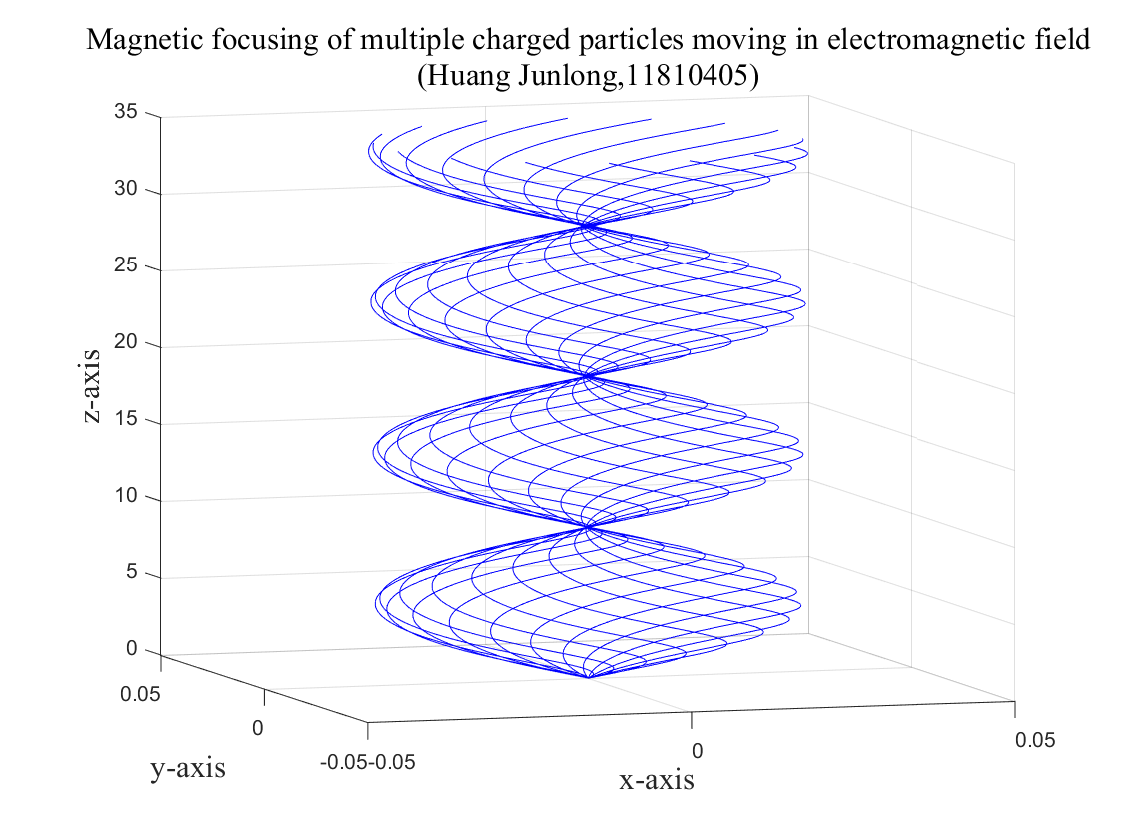
\includegraphics[width=0.9\linewidth]{Fig-1.eps}
	\caption{Magnetic focusing of multiple charged particles moving in electromagnetic field}	  
	\label{fig1} 
\end{figure}
It can be seen from the Fig. 1 that the trajectory of the overall charge is symmetrical about the z-axis and is of a spindle shape. In the z-axis direction, it will focus on a point every other distance,

\subsection{The cross section figure of $ xoy $ }
Fig. 2 shows the motion curve of the $ xoy $ section during magnetic focusing. At the same time, since the radius of motion of each charge is $ R $, then the envelope surface of their trajectory is centered on the origin and $ 2R $ is the envelope circle of radius. (As the red circle in Fig. 2)
\begin{figure}[H]   
	\centering	        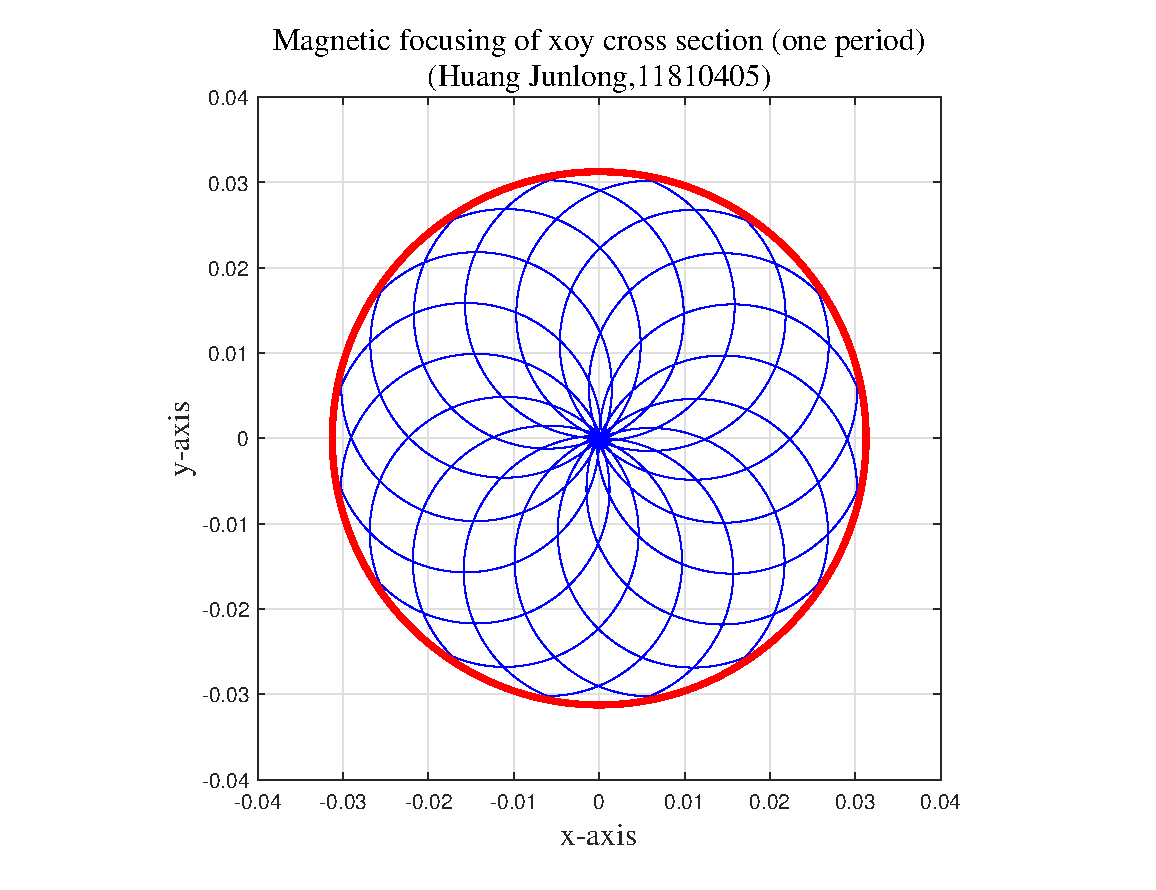
\includegraphics[width=0.9\linewidth]{Fig-2-1.eps}
	\caption{Magnetic focusing of xoy cross section (one period)}	  
	\label{fig2} 
\end{figure}

It should be noted that only one cycle is used here. This is because the $ dt $ is used as an approximation. There is a small error between the simulated trajectory and the real trajectory. When $ t $ is large, the error will accumulate in the xoy plane, resulting in not completely overlap.

Through the Equation (10) (12) (13) and parameter given in  Table 1, we can calculate the movement period and radius of the charge:
\begin{align}
R&=\dfrac{mv_{xy}}{qB}=\dfrac{0.02\times 0.1}{0.016\times 8}=0.015625\ m\\
T&=\dfrac{2\pi R}{v_{xy}}=\dfrac{2\times \pi\times 0.015625}{0.1}=0.98175\ s
\end{align}

If we draw a 5-period charge trajectory, we can see from Fig. 3 that the trajectory line becomes thicker. This is because the trajectory lines do not completely overlap due to the approximation. 

\begin{figure}[H]   
	\centering	  
	\subfloat[]{       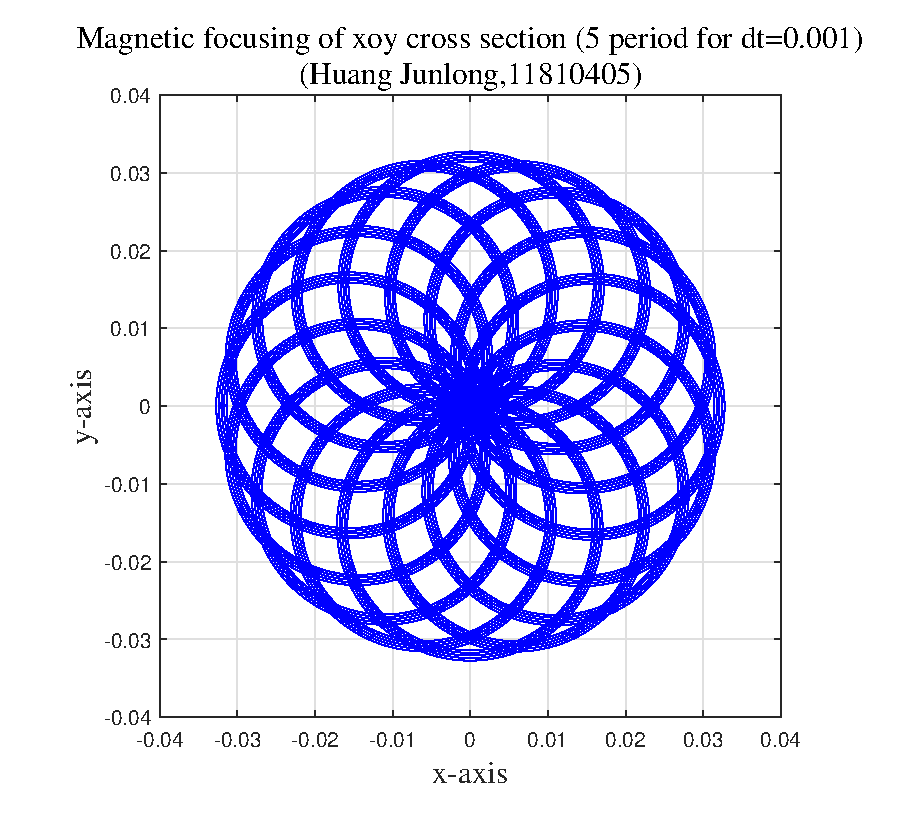
\includegraphics[width=0.45\linewidth]{Fig-3-2.eps}}    \label{1a}\hfill	  
	\subfloat[]{        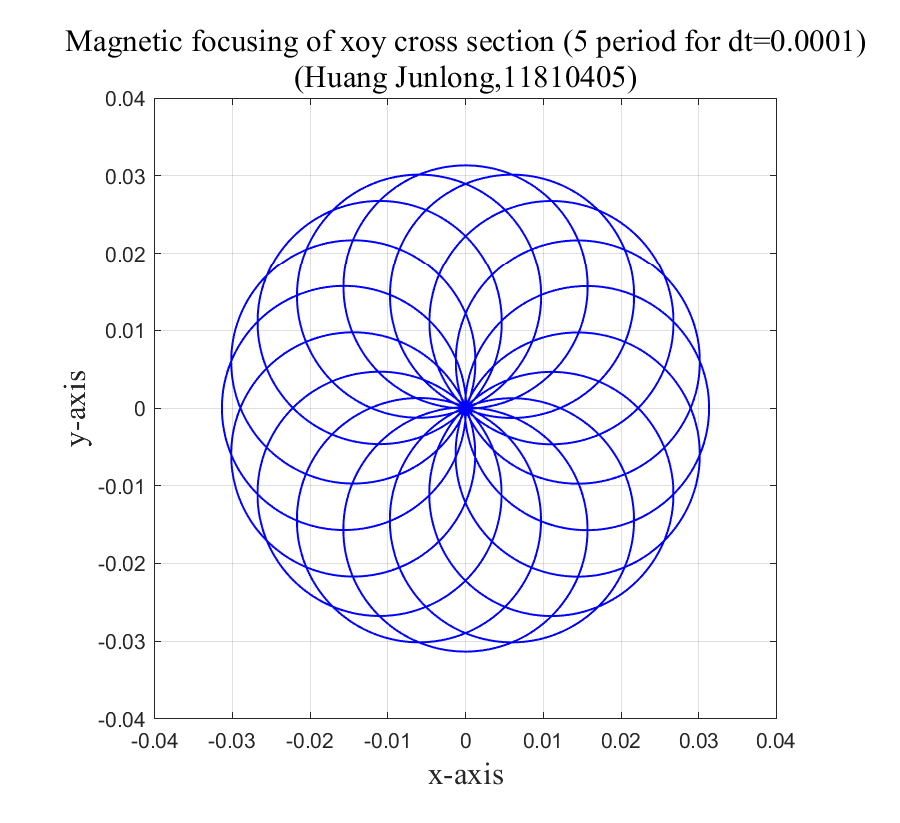
\includegraphics[width=0.45\linewidth]{Fig-3-1.eps}}    
	\label{1b}
	\caption{Magnetic focusing of xoy cross section in 5 period for : (a) time interval $ dt=0.001 $, (b) time interval $ dt=0.0001 $}	  
	\label{fig3} 
\end{figure}
However, if we change the time interval $ dt $ from $ 0.001 $ to $ 0.0001 $,  it could  be found that, the smaller the time interval dt is obtained, the more accurate the simulation result. This is in line with the actual situation. 

Then, the Fig. 4 is shown that the trajectory of 16 charges dynamic changes in a cycle which projected on the xoy plane. 
\begin{figure}[H]   
	\centering	  
	\subfloat[]{       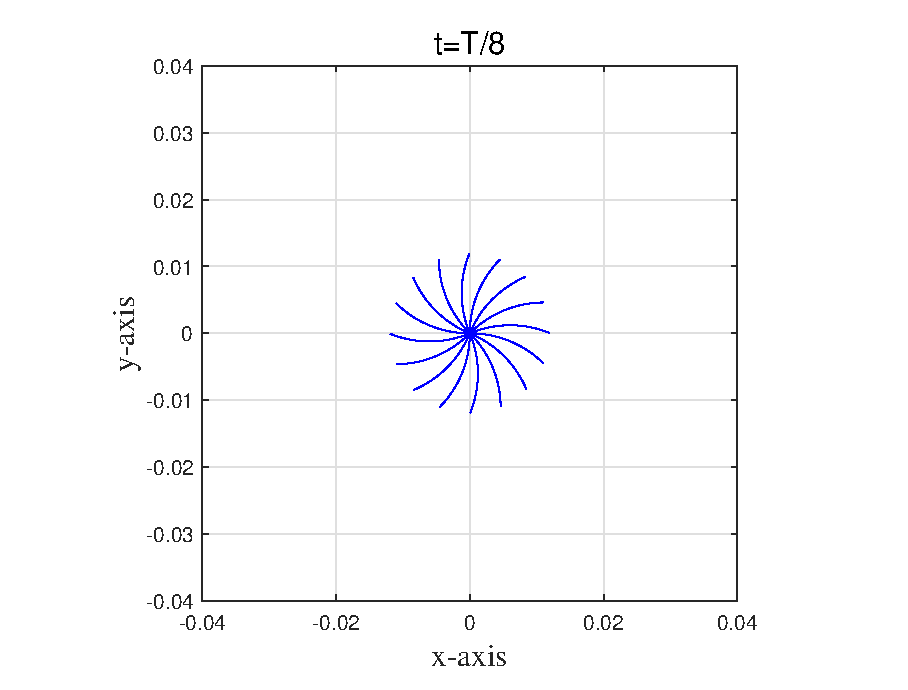
\includegraphics[width=0.22\linewidth]{Fig-4-1.eps}}    \label{4a}  
	\subfloat[]{        \includegraphics[width=0.22\linewidth]{Fig-4-2.eps}}    
	\label{4b}
	\subfloat[]{        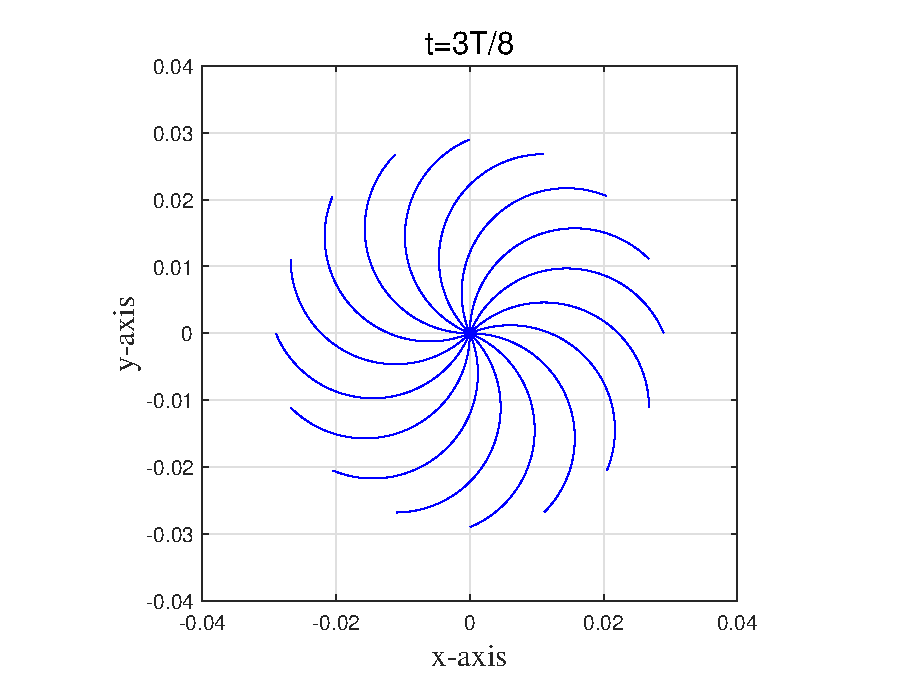
\includegraphics[width=0.22\linewidth]{Fig-4-3.eps}}    
	\label{4c}
	\subfloat[]{        \includegraphics[width=0.22\linewidth]{Fig-4-4.eps}}    
	\label{4d}\\
	\subfloat[]{        \includegraphics[width=0.22\linewidth]{Fig-4-5.eps}}    
	\label{4e}
	\subfloat[]{        \includegraphics[width=0.22\linewidth]{Fig-4-6.eps}}    
	\label{4f}
	\subfloat[]{        \includegraphics[width=0.22\linewidth]{Fig-4-7.eps}}    
	\label{4g}
	\subfloat[]{        \includegraphics[width=0.22\linewidth]{Fig-4-8.eps}}    
	\label{4h}
	\caption{Magnetic focusing of xoy cross section in one cycle: (a) $ t=\frac{1}{8}T $; (b) $ t=\frac{2}{8}T $; (c) $ t=\frac{3}{8}T $; (d) $ t=\frac{4}{8}T $; (e) $ t=\frac{5}{8}T $; (f) $ t=\frac{6}{8}T $; (g) $ t=\frac{7}{8}T $; (h) $ t=T $}.	  
	\label{fig4} 
\end{figure}


\subsection{The cross section figure of $ xoz $}
Then, we draw the cross section of $ xoz $ plane as Fig. 5.
\begin{figure}[H]   
	\centering	        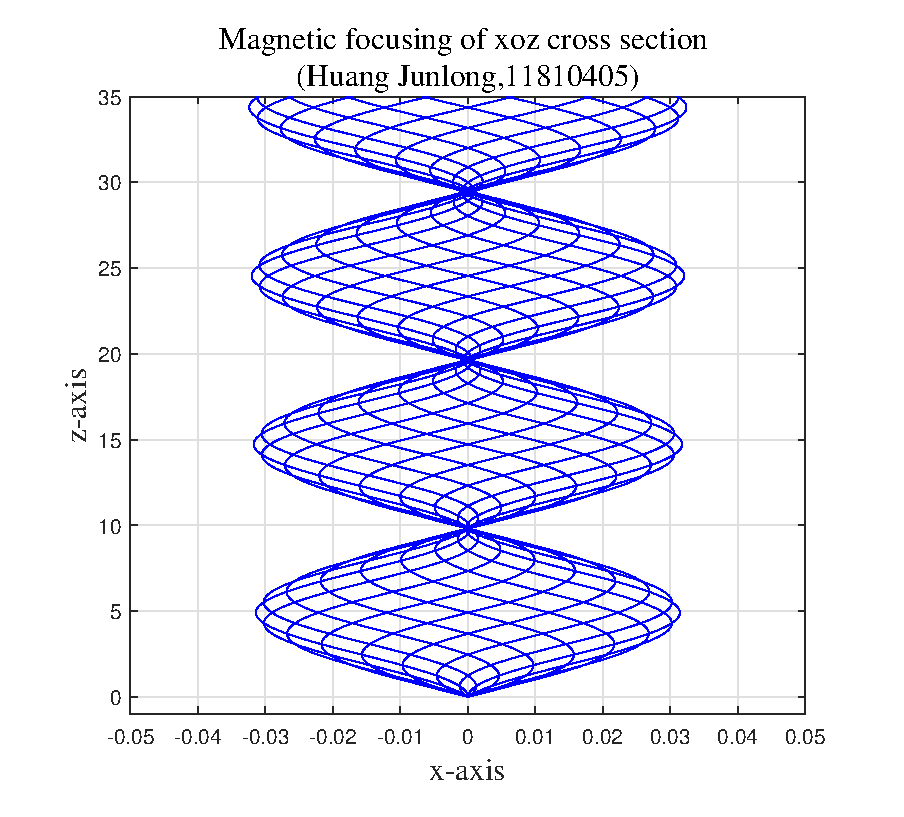
\includegraphics[width=0.6\linewidth]{Fig-5-1.eps}
	\caption{Magnetic focusing of xoz cross section}	  
	\label{fig5} 
\end{figure}

It can be clearly seen from the Fig. 5 that every time, the trajectory of each charge will refocus on a point. It can be estimated that the distance between two adjacent points is about $ 10\ m $. Actually, this distance could be calculated through equation (14) for the period $ T $ is already calculated in equation (16).
\begin{align}
L=v_z\times T=10\times 0.98175=9.8175\ m
\end{align}

Therefore, after sixteen charges leave the origin, they focus on point $ (0,9.8175) $ for the first time. Since we use $ dt $ as an approximation, the graph drawn by simulation does not pass exactly this point, but fluctuates in a small interval near this point. The size of the interval depends on the size of $ dt $. Here shows two figure for $ dt=0.001 $ and $ dt=0.0001 $:
\begin{figure}[H]   
	\centering	  
	\subfloat[]{       \includegraphics[width=0.45\linewidth]{Fig-6-3.png}}    \label{6a}\hfill	  
	\subfloat[]{        \includegraphics[width=0.45\linewidth]{Fig-6-6.png}}    
	\label{6b}
	\caption{Magnetic focusing of xoz cross section for: (a) $ dt=0.001 $; (b) $ dt=0.0001 $} 
	\label{fig6} 
\end{figure}

As $dt=0.001  $, the maximal error is less that $ 4\times 10^{-4}\ m $. As $ dt=0.0001 $, the maximal error is less that $ 5\times 10^{-5}\ m $. It is clear that the smaller the $ dt $, the smaller the error. Actually, the maximal error $ 4\times 10^{-4}\ m $ compared with the radius $ R=0.015625\ m $ and the $ L=9.8175\ m $ is already negligible.
%\begin{figure}[H]   
%	\centering	        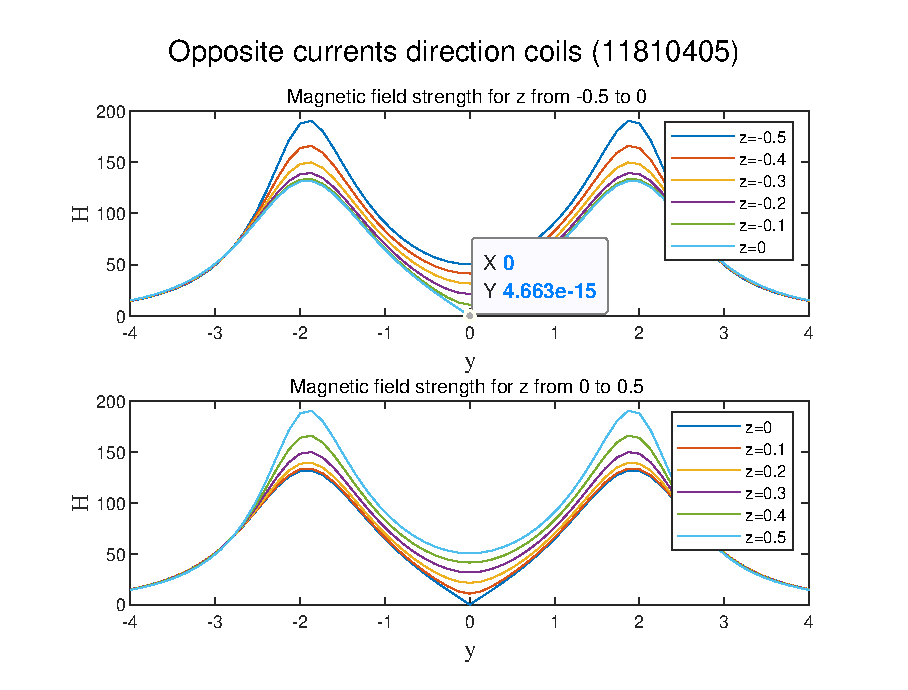
\includegraphics[width=0.9\linewidth]{F3-2.eps}
%	\caption{The vector graph of the magnetic field intensity for two current loops  between these two current loops with the opposite current direction }	  
%	\label{fig8} 
%\end{figure}

\section{Conclusion}
In a given highly symmetrical and simple example, we calculated the movement trajectory of charges in magnetic focusing through Matlab calculations. The radius of the circular motion $ R $, the period of motion $ T $, and the distance between adjacent focus points $ L $ of the drawn image all agree with the theoretical calculation. This verifies the correctness of Matlab simulation. Therefore, under more complex conditions, we can use simple Matlab simulation to replace the tedious mathematical analytical solution.

Although there is a negligible error between the simulation result and the actual result, we can reduce this error by reducing $ dt $. It should be noted that too short $ dt $ will cause a large amount of calculation leading to longer calculation time. Therefore, without affecting accuracy, this experiment uses $ dt =0.001\ s $ as the final time step.
\newpage
In addition, we find that magnetic focusing in the given situation is actually a combination of uniform circular motion and uniform linear motion. Therefore, when the charge completes a full cycle of circling movement on the $ xoy $ plane with the same period, it will re-converge in a point on the z-axis. At the same time, since there is a velocity component in the z-axis direction, the interval between the two points of charge convergence is $ L=v_z\cdot T $.

\section*{Acknowledgment}
This is the last lab of the Engineering Electromagnetic course, but the study does not end there. 
Here, I would like to thank our teacher Mr. Jia for his careful teaching since the special semester from the use of Matlab to the explanation of electromagnetic field principles and methods. We have all benefited greatly. 
And also thanks TA for reviewing our homework, teaching and answering in the tutorial time, and providing us with help and feedback in the lab.


\bibliographystyle{IEEEtran}
\bibliography{IEEEabrv,mylib}
%\begin{thebibliography}{2}

%\bibitem{IEEEhowto:kopka}
%H.~Kopka and P.~W. Daly, \emph{A Guide to \LaTeX}, 3rd~ed.\hskip 1em plus
%  0.5em minus 0.4em\relax Harlow, England: Addison-Wesley, 1999.

%\end{thebibliography}

% biography section
% 
% If you have an EPS/PDF photo (graphicx package needed) extra braces are
% needed around the contents of the optional argument to biography to prevent
% the LaTeX parser from getting confused when it sees the complicated
% \includegraphics command within an optional argument. (You could create
% your own custom macro containing the \includegraphics command to make things
% simpler here.)
%\begin{IEEEbiography}[{\includegraphics[width=1in,height=1.25in,clip,keepaspectratio]{mshell}}]{Michael Shell}
% or if you just want to reserve a space for a photo:



% You can push biographies down or up by placing
% a \vfill before or after them. The appropriate
% use of \vfill depends on what kind of text is
% on the last page and whether or not the columns
% are being equalized.

%\vfill

% Can be used to pull up biographies so that the bottom of the last one
% is flush with the other column.
%\enlargethispage{-5in}

% that's all folks
\newpage
\onecolumn 
\begin{appendices}
\section{The code of Matlab}
\end{appendices}

\begin{lstlisting}
%% This is the code for Lab 4

clc,close all,clear all                

%% Bacis parameter setting
m=0.02;                  % Set the mass
q=1.6e-2;                % Set the quantity of charge
dt=0.001;                % Set the time-step to be 0.001s
% alos 0.0001s for higher accuracy
T=0.98175;               % The period of theoretical calculation
t=0:dt:100;              % Construct the array of time. (100 T 5T)
Ex=0; Ey=0; Ez=0;        % Set the electric field vector?
Bx=0; By=0; Bz=8;        % Set the magnetic flux density vector?
vx=zeros(16,length(t));vy=vx;vz=vx;  % Construct the velocity vector?
rx=zeros(16,length(t));ry=rx;rz=rx;  % Construct the position vector?
Fx=zeros(16,length(t));Fy=Fx;Fz=Fx;  % Construct the force vector?
ax=zeros(16,length(t));ay=ax;az=ax;  % Construct the acceleration vector?

%% For 16 charge trajectories
for k=1:16
% set the init value
rx(k,1)=0;ry(k,1)=0;rz(k,1)=0;     
vx(k,1)=0.1*sin(k*pi/8);vy(k,1)=0.1*cos(k*pi/8);vz(k,1)=10;

for i=1:(length(t)-1)         % Calculate each position point 
% Calculate the acted force at position i
Fx(k,i)=q*Ex+q*(vy(k,i)*Bz-vz(k,i)*By);              
Fy(k,i)=q*Ey+q*(vz(k,i)*Bx-vx(k,i)*Bz);              
Fz(k,i)=q*Ez+q*(vx(k,i)*By-vy(k,i)*Bx);   
% Calculate the acceleration at position i
ax(k,i)=Fx(k,i)/m;                              
ay(k,i)=Fy(k,i)/m;                              
az(k,i)=Fz(k,i)/m;                              
% Calculate the velocity at position i+1 
vx(k,i+1)=vx(k,i)+ax(k,i)*dt;                        
vy(k,i+1)=vy(k,i)+ay(k,i)*dt;                        
vz(k,i+1)=vz(k,i)+az(k,i)*dt;                        
%  Calculate the position at point i+1
rx(k,i+1)=rx(k,i)+vx(k,i)*dt;         
ry(k,i+1)=ry(k,i)+vy(k,i)*dt;         
rz(k,i+1)=rz(k,i)+vz(k,i)*dt;         
end
plot3(rx(k,:),ry(k,:),rz(k,:),'blue');       
hold on
axis([-0.05,0.05,-0.05,0.05,0,35])  % set the axis
end

grid;
title({['Magnetic focusing of multiple charged particles moving in electromagnetic field'],...
['(Huang Junlong,11810405)']} ,'FontName','Times New Roman', 'fontsize', 15);           
xlabel('x-axis','FontName','Times New Roman','fontsize',15);                      
ylabel('y-axis','FontName','Times New Roman','fontsize',15);                      
zlabel('z-axis','FontName','Times New Roman','fontsize',15);      

%% The cross section of xoy plane
figure

for m=1:16
plot(rx(m,:),ry(m,:),'blue');
grid on
hold on
end

axis equal
axis([-0.04,0.04,-0.04,0.04])
title({['Magnetic focusing of xoy cross section (5 period for dt=0.001)'],...
['(Huang Junlong,11810405)']} ,'FontName','Times New Roman', 'fontsize', 15);           
% title({['Magnetic focusing of xoy cross section (t=T/8)'],...
%     ['(Huang Junlong,11810405)']} ,'FontName','Times New Roman', 'fontsize', 15); 
% title('t=T', 'fontsize', 15); 
xlabel('x-axis','FontName','Times New Roman','fontsize',15);                      
ylabel('y-axis','FontName','Times New Roman','fontsize',15);  
%% The envelope circle in xoy plane
theta = 0:0.001:2*pi;
R=0.02*0.1/0.016/8;
x=2*R.*cos(theta);
y=2*R.*sin(theta);
plot(x,y,'red','LineWidth',3)

%% The cross section of xoz plane
figure
for n=1:16
plot(rx(n,:),rz(n,:),'blue');
grid on
hold on
end
axis([-0.05,0.05,-1,35])
% title({['Magnetic focusing of xoy cross section (5 period for dt=0.001)'],...
%     ['(Huang Junlong,11810405)']} ,'FontName','Times New Roman', 'fontsize', 15);           
title({['Magnetic focusing of xoz cross section (dt=0.0001)'],...
['(Huang Junlong,11810405)']} ,'FontName','Times New Roman', 'fontsize', 15); 
xlabel('x-axis','FontName','Times New Roman','fontsize',15);                      
ylabel('z-axis','FontName','Times New Roman','fontsize',15); 

%% The datum line of xoz plane
uz=linspace(-0.05,0.05,100);
z=repmat(10*T,100);
ux=zeros(1,100);
x=linspace(9.75,9.90,100);
plot(ux,x,'red','LineWidth',2)
plot(uz,z,'red','LineWidth',2)
axis([-0.001,0.001,9.75,9.90])
%%
\end{lstlisting}


\end{document}

